\documentclass[12pt,a4paper]{book} 
\input{Configs/Configs}

\begin{document}
\renewcommand{\contentsname}{\vspace{0cm} Contenido \vspace{-2cm}}

\begin{titlepage}
\vspace*{2cm}

\noindent
\vspace*{0.5cm}
\titlefont{Machine Learning}

\vspace{1.5cm}
\epigraph{Regresión Lineal - Volumen 1}%
{ \textsc{Bustos Jordi}}
\null\vfill
\vspace*{1cm}
\noindent
\hfill
\begin{minipage}{0.7\linewidth}
    \begin{flushright}
        \printauthor
    \end{flushright}
\end{minipage}
%
\begin{minipage}{0.02\linewidth}
    \rule{1pt}{70pt}
\end{minipage}
\titlepagedecoration
\end{titlepage}

\let\cleardoublepage=\clearpage
\tableofcontents
\blankpage

\chapter{Notaciones y deficiones}
\section{¿Qué es Machine Learning?}

Machine Learning es el arte de diseñar un algoritmo tal que
pueda extraer de manera automática información de los datos. 
No, no es hacer que las máquinas piensen, al menos no por ahora. Un modelo típico de Machine Learning consiste en una formula matemática
tal que aplicada a una colección de inputs, nos devuelve el output esperado.
Las tres partes fundamentales de todo algoritmo de Machine Learning son: el modelo, los datos y el entrenamiento.
El modelo es la formula matemática (una función) que queremos hallar, los datos son la información del mundo real que usaremos para encontrar esa formula 
y el entrenamiento es el proceso de ajustar los parámetros de la formula para que se ajuste a los datos.\\

¿Por qué no consideramos esto como aprendizaje? En primer lugar no hay una instancia en la cual la máquina razone, por otro lado, 
la máquina no puede generalizar, es decir, no puede aplicar lo aprendido a situaciones nuevas. Únicamente será útil si 
los datos en los que se utilice el modelo ya entrenado son similares, en el sentido matemático, es decir, siguen una misma distribución
de probabilidad. Caso contrario el output del modelo será inútil.\\ 

Si bien es cierto que el Machine Learning hoy en día 
puede ser implementado por cualquier persona con un poco de conocimiento en programación,
al menos en un nivel muy básico, pues el software brinda las herramientas necesarias para diseñar
y entrenar modelos sin necesidad de conocer su implementación interna,
es importante tener en cuenta que es un campo de estudio muy complejo 
que requiere del conocimiento de álgebra lineal, cálculo y estadística, si queremos producir modelos útiles en el mundo real.

\section{Para quién es este libro}

Este libro es para cualquier persona que quiera aprender Machine Learning, sin importar el nivel de conocimiento matemático que posea.
Para los ejemplos y ejercicios se utilizará Python, por lo que contar con un conocimiento básico de programación en este lenguaje puede ser beneficioso.
En caso de no poseerlo, igualmente encontrará útil este libro, pues se explicará paso a paso la implementación de los algoritmos con rigurosidad matemática.

Aunque este libro no pretenda ser un manual de referencia, se espera que el lector pueda comprender los conceptos fundamentales del Machine Learning a través de una 
explicación clara y concisa, con ejemplos y un tono divulgativo, sin perder la rigurosidad y formalidad matemática necesaria para comprender los algoritmos. Además 
se proveerán implementaciones en Python de algunos de los algoritmos, para que el lector pueda experimentar con ellos y comprender su funcionamiento.

\section{Definiciones y notación}

Comencemos revisando la notación matemática que se utilizará en este libro, así como algunas definiciones y teoremas que nos serán de utilidad en el desarrollo de los temas.
Al principio puede darle la impresión de que únicamente estamos definiendo conceptos o propiedades sin relación alguna, pero tengamos en cuenta 
que los algoritmos de Machine Learning están construidos sobre las bases del álgebra lineal y el cálculo diferencial, por lo que es importante
comprender los bloques necesarios que harán que el aprendizaje de estos algoritmos sea posible, junto con su futura implementación en Python.
De más está decir que ningún algoritmo de machine learning implica un aprendizaje real de la máquina, veremos que, en general, no son más que un proceso de optimización de parametros.

\subsection{Conjuntos}

En nuestra vida cotidiana los conjuntos aparecen constantemente, aunque quizá no los reconozcamos como tal. Imaginemos por ejemplo los siguientes conjuntos:

\begin{itemize}
    \item El conjunto de los colores del arcoiris.
    \item El conjunto de sabores que podemos sentir.
    \item El conjunto de personas que conocemos.
    \item El conjunto de nuestros seguidores en redes sociales.
    \item La lista de productos que compramos hoy en el supermercado.
    \item El stock de una tienda.
\end{itemize}

Los conjuntos son unos de los pilares fundamentales de la matemática y, aunque en principio parezcan algo trivial, veremos que se irán complejizando a medida que avancemos en la teoría.
Definamos de manera formal qué es un conjunto.

\begin{definition}
    Los conjuntos son colecciones finitas o infinitas bien definida de objetos, a cada objeto en cuestión lo llamaremos elemento. 
    Al conjunto vacío lo denotaremos como $\O$.
\end{definition}

Los conjuntos los denotaremos con letras mayúsculas y pueden estar definidos por extensión (todos sus elementos listados) o por comprensión (listados a partir de una condición). 

\begin{eg}
    El conjunto de los colores del arcoiris es un conjunto cuyos elementos son $\{ rojo, naranja, amarillo, verde, azul, a\tilde{n}il, violeta \}$.\\
    En este caso el conjunto está definido por extensión.
\end{eg}

\begin{eg}
    $P = \{persona \, | \, persona \, es \, un \, ser \, humano \, que \, conozco\}$. O sea, el conjunto de los seres humanos que conozco.\\
    En este caso el conjunto está definido por comprensión.
\end{eg}

Donde ``|'' se lee como ``tal que'' y ``es alguien que conozco`` es la condición 
que deben cumplir los elementos de $P$.
Si $p$ es un elemento de $P$, o sea, $a$ pertenece a $A$ o en nuestro idioma, conozco a la persona, denotamos $p \in P$.
Por el contrario si $p$ no es un elemento de $P$, es decir, no conocemos a la persona, denotamos $p \notin P$.\\

\begin{eg}
    El conjunto de los números naturales es un conjunto cuyos elementos\\
    son $\{ 1, 2, 3, 4, \ldots \}$.
\end{eg}

\begin{eg}
    $A = \{x \, | \, x \, es \, par\}$. O sea, el conjunto de los números pares.
\end{eg}

Claramente, $A$ no puede ser listado por extensión, pues hay infinitos números pares.\\
Cuando nuestro conjunto $A$ tiene $n$ elementos, denotaremos $|A| = n$ donde $|A|$ representa el cardinal de $A$.
Si el conjunto representa todos los números en un rango de $a$ a $b$ se denota como $[a, b]$ y si no incluye a los extremos se denota como $(a, b)$.

\begin{note}
    \verb|[...]| entiendo en general por variedad o conjunto toda multiplicidad que puede ser pensada como unidad, esto es, toda colección de elementos determinados que pueden ser unidos en una totalidad mediante una ley. - Georg Cantor
\end{note}

Podemos generar un nuevo conjunto que sea la intersección de dos conjuntos $A$ y $B$. Tomando todos los elementos que pertenecen a $A$ y a $B$ simultáneamente se denota como $A \cap B$.
A su vez podemos generar un nuevo conjunto que sea la unión de dos conjuntos $A$ y $B$. Si tomamos todos los elementos que pertenecen a $A$ o a $B$ se denota como $A \cup B$.
Ejemplo de esto es si $A = \{1, 2, 3\}$ y $B = \{3, 4, 5\}$ entonces $A \cap B = \{3\}$ y $A \cup B = \{1, 2, 3, 4, 5\}$.

\subsection{Algebra lineal}

El álgebra lineal en resumidas cuentas es el campo de estudio de los vectores, las transformaciones lineales y el conjunto de reglas
que nos permiten manipularlos.

\subsubsection{Escalar, lista, vector}

\begin{definition}
    Escalar 

    Un escalar es un número perteneciente a los conjuntos $\R$  o $\C$. Una forma elegante
    de llamar a los números.
    Cuando se hable de un escalar, se asumirá que se está hablando de un número real, a menos que se 
    especifique lo contrario y se lo notará en itálica.
\end{definition}

Ejemplos concretos de escalares son los números $10$, $4i$, $-3.5$, $\pi$, entre otros.

\begin{definition}
    Lista 

    Supongamos $n$ es un número positivo. Una lista de longitud $n$ es una colección ordenada de $n$ elementos 
    (que pueden ser escalares, vectores o cualquier entidad matemática) rodeados por paréntesis y separados por comas.
    Una lista de longitud $n$ se ve de la siguiente forma:
    \begin{equation}
        (x_1, x_2, \ldots, x_n)
    \end{equation}

    Además dos listas son iguales si y solo si sus elementos correspondientes son iguales.
\end{definition}

Por ejemplo $(1, 2, 3)$ y $(1, 2, 3)$ son listas iguales, mientras que $(1, 2, 3)$ y $(1, 3, 2)$ no lo son. Todas listas de longitud 3.

\begin{definition}
    $\K^n$
    
    Si consideramos $\K$ como $\R$ o $\C$ entonces $\K^n$ es el conjunto de todas las listas de longitud $n$ conformadas por elementos de $\K$.
    $$ \K^n = \{(x_1, x_2, \ldots, x_n) \,|\, x_i \in \mathbb{K}, \forall i = 1, 2, \ldots, n\} $$.
\end{definition}

$\forall $ es un símbolo matemático que se lee como ``para todo'' y | es un símbolo matemático que se lee como ``tal que'', según la bibliografía puede usarse el símbolo : para representar lo mismo.

Entonces, el conjunto $ \K^n = \{(x_1, x_2, \ldots, x_n) \,|\, x_i \in \mathbb{K}, \forall i = 1, 2, \ldots, n\}$
se lee como ``el conjunto de todas las listas de longitud $n$ tal que cada $x_i$ para todo $i$ entre $1$ y $n$, $x_i pertenece a \K$''.
Por ejemplo, $\R^3$ es el conjunto de todas las listas de longitud 3 de números reales. $\R^3 = \{(x, y, z) \,|\, x, y, z \in \R\}$.

\begin{definition}
    Vector
    
    Un vector es cualquier objeto que respete la suma y la multiplicación por un escalar generando otro objeto de su misma clase. Un vector de longitud $n$ es un elemento de $\mathbb{K}^n$. Los denotaremos con letras minúsculas en negrita. Y usaremos la notación $\mathbf{x}_i$ para referirnos al $i$-ésimo elemento de un vector.
\end{definition}

Los vectores geométricos pueden ser visualizados como puntos o flechas en un espacio $n$-dimensional.\\
Una notación que además sera conveniente para simplifcar la escritura es la sumatoria y la productoria. Supongamos que tenemos un conjunto de números $\mathbb{x} = \{x_1, x_2, \ldots, x_n\}$ y queremos sumarlos,
entonces podemos escribirlo como $$\sum_{i=0}^{n} x_i = x_0 + x_1 + \ldots + x_n$$ que se lee como ``la suma de $x_i$ desde $i=0$ hasta $i=n$''.
De igual forma si queremos multiplicarlos, podemos escribirlo como $$\prod_{i=0}^{n} x_i = x_0 x_1 \ldots x_n$$ que se lee como ``el producto de $x_i$ desde $i=0$ hasta $i=n$''.

\begin{figure}[htbp]
    \centering
    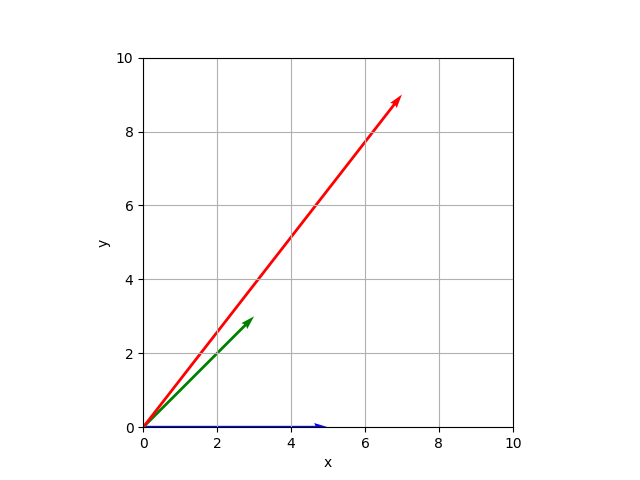
\includegraphics[width=0.4\textwidth]{Images/1/vectors.png}
    \hspace{2cm} 
    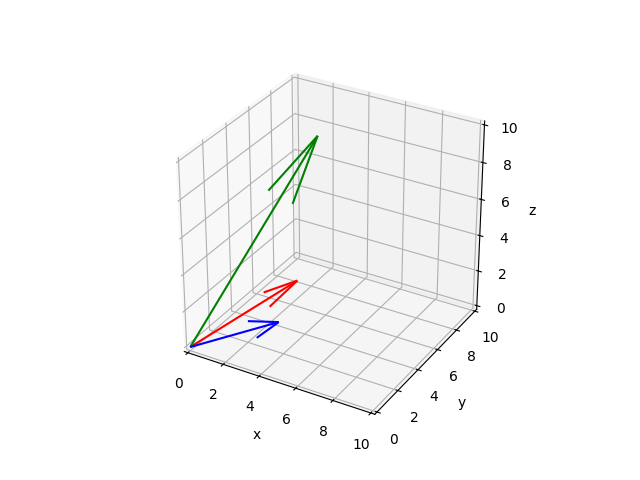
\includegraphics[width=0.4\textwidth]{Images/1/vectors_3d.png}
    \caption{Visualización de vectores en $\R^2$ y $\R^3$ respectivamente.}
    \label{fig:vectores_en_el_plano}
\end{figure}

La suma entre vectores está bien definida si los dos vectores tienen la misma cantidad de elementos y se realiza componente a componente de la siguiente forma:\\
Si $\mathbf{u} = (u_1, u_2, \ldots, u_n)$ y $\mathbf{v} = (v_1, v_2, \ldots, v_n)$ entonces $\mathbf{u} + \mathbf{v} = (u_1 + v_1, u_2 + v_2, \ldots, u_n + v_n)$. 
La resta se puede pensar como la suma de un vector con el opuesto del otro vector.\\
La multiplicación por un escalar está dada por $\alpha \mathbf{u} = (\alpha u_1, \alpha u_2, \ldots, \alpha u_n)$. 

\begin{figure}[htbp]
    \centering
    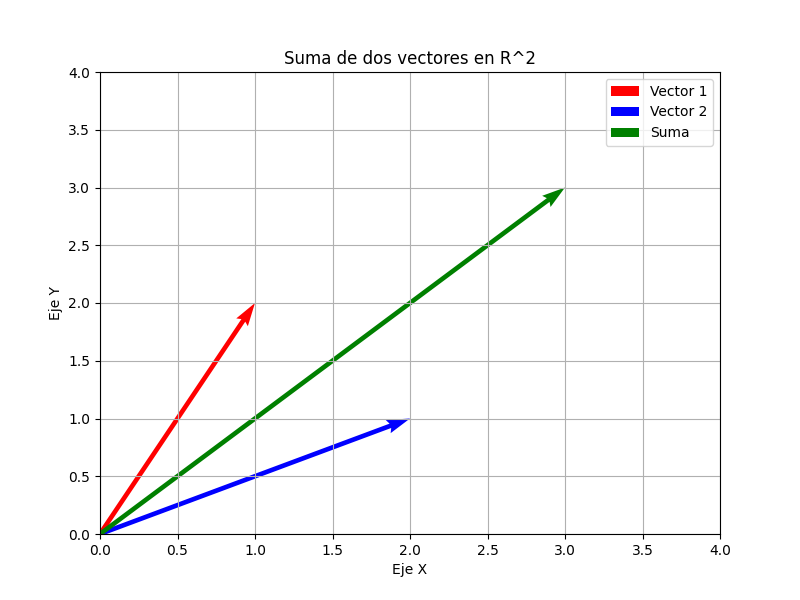
\includegraphics[width=0.6\textwidth]{Images/1/sum_of_two_vectors.png}
    \caption{La suma de dos vectores resulta en la diagonal del paralelogramo que se forma con ellos.}
    \label{fig:suma_de_vectores}
\end{figure}

\subsection{Examples 2}

\newpage\thispagestyle{empty}\blankpage

\chapter{Examples II}
\section{Examplessss}

I put this chapter to show how Index works\\

You can put your own bibs file and also change language for english in "Formats.tex" you will find the index configs.\\

\lipsum[1-6]





You can delete that line and get the original typography of latex.
\newpage\thispagestyle{empty}\blankpage


\blankpage
\bibliographystyle{unsrt}
\bibliography{references}
\nocite{*}



\end{document}